\documentclass{standalone}
\usepackage{tikz}
\usetikzlibrary{patterns, positioning}
\usepackage[sfdefault]{ClearSans} %% option 'sfdefault' activates Clear Sans as the default text font
\usepackage[T1]{fontenc}

\begin{document}
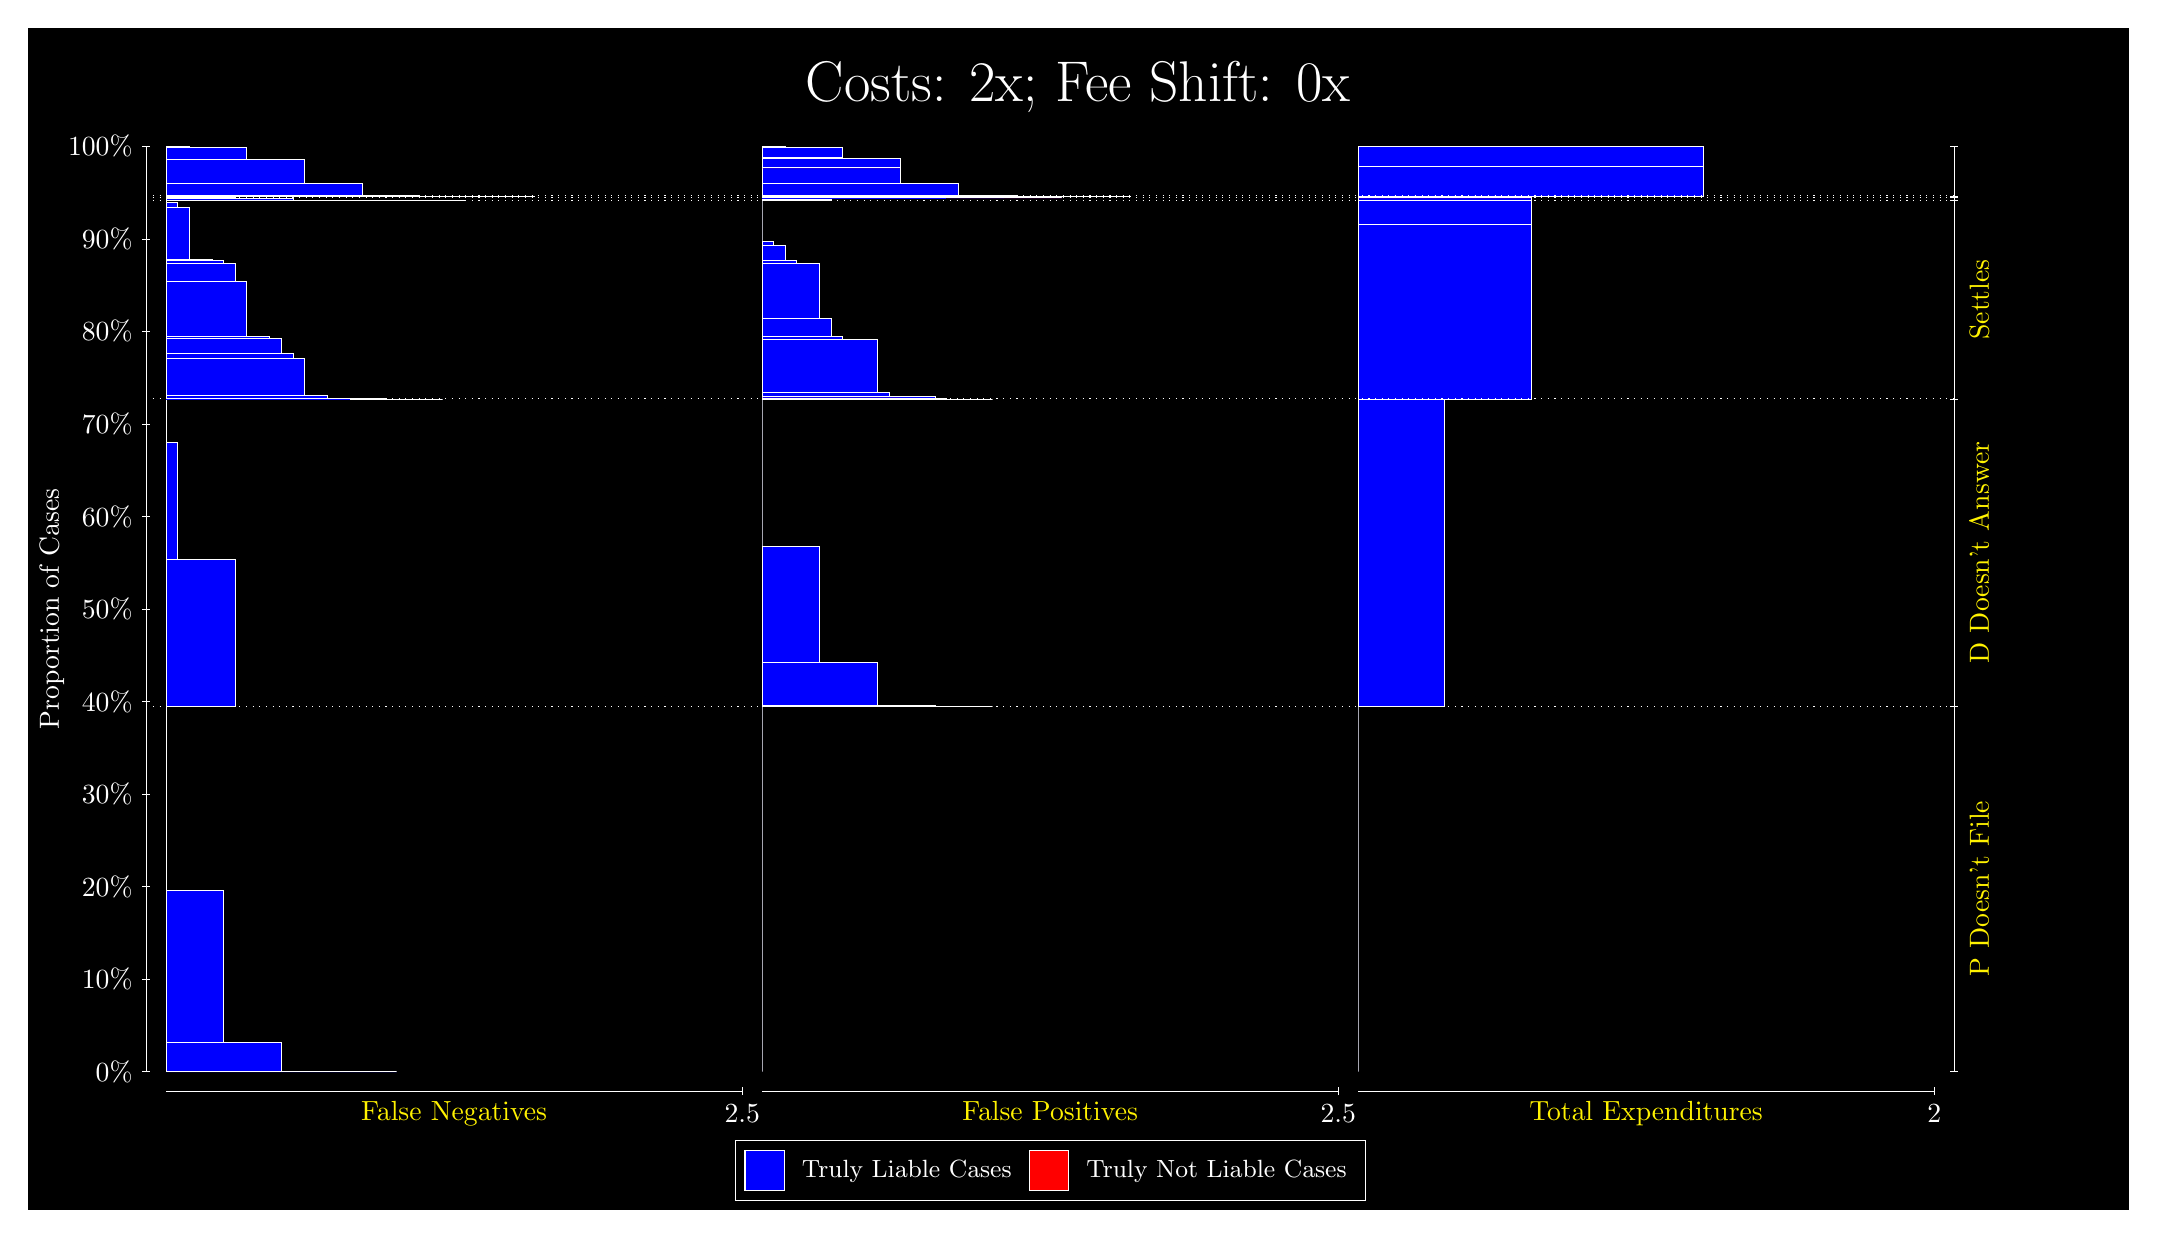
\begin{tikzpicture}
\draw[fill=black] (0,0) rectangle (26.667,15);
\draw[text=white] (0,13.5) rectangle (26.667,15) node[midway] {\huge Costs: 2x; Fee Shift: 0x};
\draw[white, very thin] (1.5,1.75) -- (1.5,13.5);
\node[rotate=90, text=white, anchor=center] at (0.3, 7.625) {Proportion of Cases};
\draw[white, very thin] (1.45,1.75) -- (1.55,1.75);
\node[text=white, anchor=east] at (1.45, 1.75) {0\%};
\draw[white, very thin] (1.45,2.925) -- (1.55,2.925);
\node[text=white, anchor=east] at (1.45, 2.925) {10\%};
\draw[white, very thin] (1.45,4.1) -- (1.55,4.1);
\node[text=white, anchor=east] at (1.45, 4.1) {20\%};
\draw[white, very thin] (1.45,5.275) -- (1.55,5.275);
\node[text=white, anchor=east] at (1.45, 5.275) {30\%};
\draw[white, very thin] (1.45,6.45) -- (1.55,6.45);
\node[text=white, anchor=east] at (1.45, 6.45) {40\%};
\draw[white, very thin] (1.45,7.625) -- (1.55,7.625);
\node[text=white, anchor=east] at (1.45, 7.625) {50\%};
\draw[white, very thin] (1.45,8.8) -- (1.55,8.8);
\node[text=white, anchor=east] at (1.45, 8.8) {60\%};
\draw[white, very thin] (1.45,9.975) -- (1.55,9.975);
\node[text=white, anchor=east] at (1.45, 9.975) {70\%};
\draw[white, very thin] (1.45,11.15) -- (1.55,11.15);
\node[text=white, anchor=east] at (1.45, 11.15) {80\%};
\draw[white, very thin] (1.45,12.325) -- (1.55,12.325);
\node[text=white, anchor=east] at (1.45, 12.325) {90\%};
\draw[white, very thin] (1.45,13.5) -- (1.55,13.5);
\node[text=white, anchor=east] at (1.45, 13.5) {100\%};

\draw[white, very thin] (24.457,1.75) -- (24.457,13.5);
\draw[white, very thin] (24.407,1.75) -- (24.507,1.75);
\node[anchor=west] at (24.407, 1.75) {};
\draw[white, very thin] (24.407,6.3903) -- (24.507,6.3903);
\node[anchor=west] at (24.407, 6.3903) {};
\draw[white, very thin] (24.407,10.293) -- (24.507,10.293);
\node[anchor=west] at (24.407, 10.293) {};
\draw[white, very thin] (24.407,12.815) -- (24.507,12.815);
\node[anchor=west] at (24.407, 12.815) {};
\draw[white, very thin] (24.407,12.847) -- (24.507,12.847);
\node[anchor=west] at (24.407, 12.847) {};
\draw[white, very thin] (24.407,12.87) -- (24.507,12.87);
\node[anchor=west] at (24.407, 12.87) {};
\draw[white, very thin] (24.407,13.5) -- (24.507,13.5);
\node[anchor=west] at (24.407, 13.5) {};

\draw[white, very thin, fill=blue] (1.75,1.75) rectangle (4.6775,1.75);
\draw[white, very thin, fill=blue] (1.75,1.75) rectangle (3.9457,1.7531);
\draw[white, very thin, fill=blue] (1.75,1.7531) rectangle (3.2138,2.117);
\draw[white, very thin, fill=blue] (1.75,2.117) rectangle (2.4819,4.0547);
\draw[white, very thin, fill=red] (1.75,4.0547) rectangle (1.75,4.0547);
\draw[white, very thin, fill=blue] (1.75,4.0547) rectangle (1.75,6.3903);
\draw[white, very thin, fill=blue] (1.75,6.3903) rectangle (2.6283,8.2576);
\draw[white, very thin, fill=blue] (1.75,8.2576) rectangle (1.8964,9.7378);
\draw[white, very thin, fill=red] (1.75,9.7378) rectangle (1.75,9.7378);
\draw[white, very thin, fill=blue] (1.75,9.7378) rectangle (1.75,10.293);
\draw[white, very thin, fill=blue] (1.75,10.293) rectangle (5.2631,10.293);
\draw[white, very thin, fill=blue] (1.75,10.293) rectangle (4.6775,10.293);
\draw[white, very thin, fill=blue] (1.75,10.293) rectangle (4.5312,10.294);
\draw[white, very thin, fill=blue] (1.75,10.294) rectangle (4.092,10.295);
\draw[white, very thin, fill=blue] (1.75,10.295) rectangle (3.9457,10.304);
\draw[white, very thin, fill=blue] (1.75,10.304) rectangle (3.7993,10.34);
\draw[white, very thin, fill=blue] (1.75,10.34) rectangle (3.5065,10.811);
\draw[white, very thin, fill=blue] (1.75,10.811) rectangle (3.3602,10.871);
\draw[white, very thin, fill=blue] (1.75,10.871) rectangle (3.2138,11.061);
\draw[white, very thin, fill=blue] (1.75,11.061) rectangle (3.0674,11.089);
\draw[white, very thin, fill=blue] (1.75,11.089) rectangle (2.7746,11.792);
\draw[white, very thin, fill=blue] (1.75,11.792) rectangle (2.6283,12.017);
\draw[white, very thin, fill=blue] (1.75,12.017) rectangle (2.4819,12.059);
\draw[white, very thin, fill=blue] (1.75,12.059) rectangle (2.3355,12.06);
\draw[white, very thin, fill=blue] (1.75,12.06) rectangle (2.0428,12.731);
\draw[white, very thin, fill=blue] (1.75,12.731) rectangle (1.8964,12.788);
\draw[white, very thin, fill=red] (1.75,12.788) rectangle (1.75,12.788);
\draw[white, very thin, fill=blue] (1.75,12.788) rectangle (1.75,12.815);
\draw[white, very thin, fill=blue] (1.75,12.815) rectangle (5.5558,12.815);
\draw[white, very thin, fill=blue] (1.75,12.815) rectangle (4.8239,12.815);
\draw[white, very thin, fill=blue] (1.75,12.815) rectangle (4.092,12.817);
\draw[white, very thin, fill=blue] (1.75,12.817) rectangle (3.3602,12.838);
\draw[white, very thin, fill=blue] (1.75,12.838) rectangle (2.6283,12.847);
\draw[white, very thin, fill=red] (1.75,12.847) rectangle (1.75,12.847);
\draw[white, very thin, fill=blue] (1.75,12.847) rectangle (2.6283,12.856);
\draw[white, very thin, fill=blue] (1.75,12.856) rectangle (1.8964,12.87);
\draw[white, very thin, fill=red] (1.75,12.87) rectangle (1.75,12.87);
\draw[white, very thin, fill=blue] (1.75,12.87) rectangle (1.75,12.87);
\draw[white, very thin, fill=blue] (1.75,12.87) rectangle (6.4341,12.87);
\draw[white, very thin, fill=blue] (1.75,12.87) rectangle (5.7022,12.87);
\draw[white, very thin, fill=blue] (1.75,12.87) rectangle (4.9703,12.879);
\draw[white, very thin, fill=blue] (1.75,12.879) rectangle (4.2384,13.025);
\draw[white, very thin, fill=blue] (1.75,13.025) rectangle (3.5065,13.341);
\draw[white, very thin, fill=blue] (1.75,13.341) rectangle (2.7746,13.488);
\draw[white, very thin, fill=blue] (1.75,13.488) rectangle (2.0428,13.5);
\draw[white, very thin, fill=red] (1.75,13.5) rectangle (1.75,13.5);
\draw[white, very thin, fill=blue] (1.75,13.5) rectangle (1.75,13.5);
\draw[white, very thin, fill=red] (9.3189,1.75) rectangle (9.3189,1.75);
\draw[white, very thin, fill=blue] (9.3189,1.75) rectangle (9.3189,6.3903);
\draw[white, very thin, fill=red] (9.3189,6.3903) rectangle (12.246,6.3903);
\draw[white, very thin, fill=blue] (9.3189,6.3903) rectangle (12.246,6.3903);
\draw[white, very thin, fill=blue] (9.3189,6.3903) rectangle (11.515,6.4049);
\draw[white, very thin, fill=blue] (9.3189,6.4049) rectangle (10.783,6.9454);
\draw[white, very thin, fill=blue] (9.3189,6.9454) rectangle (10.051,8.4257);
\draw[white, very thin, fill=blue] (9.3189,8.4257) rectangle (9.3189,10.293);
\draw[white, very thin, fill=red] (9.3189,10.293) rectangle (12.246,10.293);
\draw[white, very thin, fill=blue] (9.3189,10.293) rectangle (12.246,10.293);
\draw[white, very thin, fill=red] (9.3189,10.293) rectangle (11.661,10.293);
\draw[white, very thin, fill=blue] (9.3189,10.293) rectangle (11.661,10.294);
\draw[white, very thin, fill=blue] (9.3189,10.294) rectangle (11.515,10.32);
\draw[white, very thin, fill=red] (9.3189,10.32) rectangle (11.075,10.32);
\draw[white, very thin, fill=blue] (9.3189,10.32) rectangle (11.075,10.32);
\draw[white, very thin, fill=blue] (9.3189,10.32) rectangle (10.929,10.377);
\draw[white, very thin, fill=blue] (9.3189,10.377) rectangle (10.783,11.048);
\draw[white, very thin, fill=red] (9.3189,11.048) rectangle (10.49,11.048);
\draw[white, very thin, fill=blue] (9.3189,11.048) rectangle (10.49,11.049);
\draw[white, very thin, fill=blue] (9.3189,11.049) rectangle (10.344,11.091);
\draw[white, very thin, fill=blue] (9.3189,11.091) rectangle (10.197,11.316);
\draw[white, very thin, fill=blue] (9.3189,11.316) rectangle (10.051,12.019);
\draw[white, very thin, fill=blue] (9.3189,12.019) rectangle (9.758,12.047);
\draw[white, very thin, fill=blue] (9.3189,12.047) rectangle (9.6116,12.237);
\draw[white, very thin, fill=blue] (9.3189,12.237) rectangle (9.4652,12.297);
\draw[white, very thin, fill=blue] (9.3189,12.297) rectangle (9.3189,12.815);
\draw[white, very thin, fill=red] (9.3189,12.815) rectangle (10.197,12.815);
\draw[white, very thin, fill=blue] (9.3189,12.815) rectangle (10.197,12.825);
\draw[white, very thin, fill=blue] (9.3189,12.825) rectangle (9.4652,12.845);
\draw[white, very thin, fill=blue] (9.3189,12.845) rectangle (9.3189,12.847);
\draw[white, very thin, fill=red] (9.3189,12.847) rectangle (13.125,12.847);
\draw[white, very thin, fill=blue] (9.3189,12.847) rectangle (13.125,12.847);
\draw[white, very thin, fill=blue] (9.3189,12.847) rectangle (12.393,12.847);
\draw[white, very thin, fill=blue] (9.3189,12.847) rectangle (11.661,12.848);
\draw[white, very thin, fill=blue] (9.3189,12.848) rectangle (10.929,12.861);
\draw[white, very thin, fill=blue] (9.3189,12.861) rectangle (10.197,12.87);
\draw[white, very thin, fill=red] (9.3189,12.87) rectangle (14.003,12.87);
\draw[white, very thin, fill=blue] (9.3189,12.87) rectangle (14.003,12.87);
\draw[white, very thin, fill=red] (9.3189,12.87) rectangle (13.271,12.87);
\draw[white, very thin, fill=blue] (9.3189,12.87) rectangle (13.271,12.87);
\draw[white, very thin, fill=red] (9.3189,12.87) rectangle (12.539,12.87);
\draw[white, very thin, fill=blue] (9.3189,12.87) rectangle (12.539,12.882);
\draw[white, very thin, fill=blue] (9.3189,12.882) rectangle (11.807,13.028);
\draw[white, very thin, fill=red] (9.3189,13.028) rectangle (11.807,13.028);
\draw[white, very thin, fill=blue] (9.3189,13.028) rectangle (11.807,13.029);
\draw[white, very thin, fill=blue] (9.3189,13.029) rectangle (11.075,13.229);
\draw[white, very thin, fill=red] (9.3189,13.229) rectangle (11.075,13.229);
\draw[white, very thin, fill=blue] (9.3189,13.229) rectangle (11.075,13.345);
\draw[white, very thin, fill=blue] (9.3189,13.345) rectangle (10.344,13.364);
\draw[white, very thin, fill=blue] (9.3189,13.364) rectangle (10.344,13.491);
\draw[white, very thin, fill=blue] (9.3189,13.491) rectangle (9.6116,13.491);
\draw[white, very thin, fill=blue] (9.3189,13.491) rectangle (9.6116,13.5);
\draw[white, very thin, fill=blue] (9.3189,13.5) rectangle (9.3189,13.5);
\draw[white, very thin, fill=red] (16.888,1.75) rectangle (16.888,1.75);
\draw[white, very thin, fill=blue] (16.888,1.75) rectangle (16.888,6.3903);
\draw[white, very thin, fill=red] (16.888,6.3903) rectangle (17.986,6.3903);
\draw[white, very thin, fill=blue] (16.888,6.3903) rectangle (17.986,10.293);
\draw[white, very thin, fill=red] (16.888,10.293) rectangle (19.083,10.293);
\draw[white, very thin, fill=blue] (16.888,10.293) rectangle (19.083,12.509);
\draw[white, very thin, fill=red] (16.888,12.509) rectangle (19.083,12.509);
\draw[white, very thin, fill=blue] (16.888,12.509) rectangle (19.083,12.815);
\draw[white, very thin, fill=red] (16.888,12.815) rectangle (19.083,12.815);
\draw[white, very thin, fill=blue] (16.888,12.815) rectangle (19.083,12.847);
\draw[white, very thin, fill=red] (16.888,12.847) rectangle (19.083,12.847);
\draw[white, very thin, fill=blue] (16.888,12.847) rectangle (19.083,12.87);
\draw[white, very thin, fill=red] (16.888,12.87) rectangle (21.279,12.87);
\draw[white, very thin, fill=blue] (16.888,12.87) rectangle (21.279,13.248);
\draw[white, very thin, fill=red] (16.888,13.248) rectangle (21.279,13.248);
\draw[white, very thin, fill=blue] (16.888,13.248) rectangle (21.279,13.5);
\draw[white, dotted] (1.5,6.3903) -- (24.457,6.3903);
\draw[white, dotted] (1.5,10.293) -- (24.457,10.293);
\draw[white, dotted] (1.5,12.815) -- (24.457,12.815);
\draw[white, dotted] (1.5,12.847) -- (24.457,12.847);
\draw[white, dotted] (1.5,12.87) -- (24.457,12.87);
\draw[white, very thin] (1.75,1.5) -- (9.0689,1.5);
\node[text=yellow, anchor=north] at (5.4094, 1.5) {False Negatives};
\draw[white, very thin] (9.0689,1.45) -- (9.0689,1.55);
\node[text=white, anchor=north] at (9.0689, 1.45) {2.5};

\draw[white, very thin] (9.3189,1.5) -- (16.638,1.5);
\node[text=yellow, anchor=north] at (12.978, 1.5) {False Positives};
\draw[white, very thin] (16.638,1.45) -- (16.638,1.55);
\node[text=white, anchor=north] at (16.638, 1.45) {2.5};

\draw[white, very thin] (16.888,1.5) -- (24.207,1.5);
\node[text=yellow, anchor=north] at (20.547, 1.5) {Total Expenditures};
\draw[white, very thin] (24.207,1.45) -- (24.207,1.55);
\node[text=white, anchor=north] at (24.207, 1.45) {2};

\node[text=yellow, centered, rotate=90] at (24.777, 4.0701) {P Doesn't File};
\node[text=yellow, centered, rotate=90] at (24.777, 8.3416) {D Doesn't Answer};
\node[text=yellow, centered, rotate=90] at (24.777, 11.554) {Settles};




\draw (12.978300999999998,1.5) node[draw=none] (baseCoordinate) {};
\begin{scope}[align=center]
        \matrix[scale=0.5, draw=white, below=0.5cm of baseCoordinate, nodes={draw}, column sep=0.1cm]{
            \node[rectangle, draw, minimum width=0.5cm, minimum height=0.5cm, fill=blue] {}; &
            \node[draw=none, font=\small, text=white] (B) {Truly Liable Cases}; &
            \node[rectangle, draw, minimum width=0.5cm, minimum height=0.5cm, fill=red] {}; &
            \node[draw=none, font=\small, text=white] (B) {Truly Not Liable Cases}; \\
            };
\end{scope}

\end{tikzpicture}
\end{document}